\chapter{针对模型框架层的新型恶意模型攻击分析与检测框架}
\section{引言}
近年来，随着 AI 技术的快速演进，各行业加速推进智能化与自动化转型，AI 模型已成为支撑智能应用的核心部件。当前大量 AI 软件均以预训练模型作为基础能力模块，然而，随着模型规模持续扩大以及训练数据质量要求不断提升，模型训练所需的算力与数据成本显著攀升。在此背景下，开发者广泛采用开源预训练模型以降低研发门槛与部署成本，从而推动了 \code{Hugging Face}、\code{TensorFlow Hub} 等开源模型共享平台的快速发展。尽管这种开箱即用的模型共享模式显著提升了 AI 应用的开发效率，但其同时引入了严峻的供应链安全风险。AI 模型通常包含复杂的参数结构与计算图逻辑，并以二进制格式进行分发，模型内部实现细节对使用者而言高度不透明。攻击者可利用这种结构与分发形式上的不透明性，将恶意逻辑或行为隐蔽嵌入模型之中。当受害者在下游系统中加载并执行此类模型时，相关恶意行为将在模型推理过程中被自动触发，从而在无显式漏洞利用的情况下对 AI 系统造成实质性威胁。

模型框架层作为承载 AI 模型训练与推理的核心运行基础，模型供应链的安全性直接决定了整个模型框架层和上层应用层的可靠性。目前，学术界与工业界针对 AI 系统模型供应链的安全研究都集中于传统的恶意模型，即局限于对抗性攻击、模型提取以及数据投毒等传统安全领域，而针对模型共享机制及模型文件本身作为恶意软件载体的相关安全研究相对匮乏。现有针对恶意模型的攻击方法主要通过篡改或替换模型权重参数来实现，此类方案不仅会导致模型精度显著下降，且极易被常规的完整性校验机制所捕获。另一方面，针对模型反序列化漏洞的攻击通常聚焦于 \code{PyTorch} 等框架所采用的、已知存在设计缺陷的 \code{pickle} 序列化机制，该类漏洞已被广泛研究并催生了如 \code{Fickling} 等成熟的安全扫描工具~\cite{fickling_defcon_2021}。相比之下，\code{TensorFlow}等框架采用了安全性更高的\code{Protobuf}序列化格式，有效规避了传统反序列化漏洞，在数据结构层面具备更强的类型安全性。然而，其框架内部大量合法 API 所隐含的系统级能力及其潜在安全风险，长期缺乏系统性分析。

针对上述研究空白，本章聚焦于 AI 系统模型框架层的供应链安全问题，对模型供应链进行系统化分析，对其展开了系统性的脆弱性分析与威胁建模。本研究首次揭示\code{TensorFlow} 等主流框架在提供模型构建与训练能力的同时，其部分合法 API 具备隐式的系统能力，例如文件读取、文件写入以及网络通信等操作。这些能力在正常使用场景下服务于数据处理与分布式训练，但在特定条件下可被滥用以构造隐蔽的恶意模型。本研究将这种利用框架原生合法 API 隐藏能力构造攻击模型的新型攻击范式定义为 \code{TensorAbuse} 攻击。围绕该攻击范式，本研究开展了系统性分析，不仅识别出 \code{TensorFlow} 框架中 31 个可被滥用的关键 API，构建了完整的攻击原语体系，同时设计并实现了一套针对该类恶意模型的自动化检测工具。具体来说，本章节主要涵盖以下四个方面的创新性工作：

首先，本研究首次提出了一类针对模型框架层的原生 API 滥用攻击—— \code{TensorAbuse} 攻击。与传统依赖内存破坏或系统漏洞利用的攻击不同，\code{TensorAbuse} 并不依赖底层漏洞，而是直接滥用框架内合法 API 所具备的隐藏系统能力（如文件读取、网络通信等），并将其嵌入为模型计算图中的持久化操作节点。当模型在推理阶段被加载与执行时，相关恶意操作将自动触发，实现持久化与隐蔽化执行，具有较高的规避性与破坏潜力。

其次，在技术方法层面，本研究提出了一套 \code{TensorAbuse} 攻击自动化分析与提取框架，核心包括两个关键步骤：API持久化可行性分析与持久化API隐藏能力挖掘。针对底层框架逻辑错综复杂且官方文档缺乏API持久化属性说明的技术挑战，本研究设计了名为 \code{PersistExt} 的持久化API自动提取技术。该技术采用启发式特征匹配策略，结合抽象语法树对 Python 前端源码进行结构化解析，并利用 \code{CodeQL} 对C++后端底层算子实现自动化污点追踪与跨语言映射，从而实现了对 \code{TensorFlow} 框架持久化API的高效提取。进一步地，在 API 隐藏能力挖掘阶段，面对框架API基数庞大及跨语言调用链复杂的瓶颈，本研究提出了名为 \code{CapAnalysis} 的新型隐蔽能力分析技术。该技术创新性地引入大语言模型进行深层代码语义理解与行为定性分析，通过构建基于思维链（Chain-of-Thought, CoT）的结构化提示工程，对大规模 API 进行自动化语义分析，从而实现对潜在隐藏能力的高精度提取。

在威胁建模与评估方面，本研究对 \code{TensorFlow 2.15.0} 版本的完整源码树进行了详尽的 API 分析，共提取出 1083 个可持久化至模型文件的 API。在隐蔽能力提取阶段，通过能力筛选识别出 31 个可被滥用于攻击构造的高风险 API。基于这些 API 能力，本研究构建了五类基础攻击原语，并进一步组合形成四类具有实质破坏能力的恶意攻击行为。实验结果表明，上述攻击可在不影响模型精度的前提下无缝嵌入至正常模型之中，并能够有效绕过当前业界较为先进的模型扫描工具 \code{ModelScan} 的检测~\cite{modelscan_github_2024}。

最后，在安全防护与生态治理层面，鉴于现有的安全检测基建无法有效应对原生 API 滥用这一新型攻击面，本研究自主研发并开源了一套专门针对恶意模型的定制化安全扫描防御框架，有效加固了AI系统模型框架层的运行底座。同时，本研究恪守负责任的漏洞披露原则，已将所有核心安全发现与技术细节向 \code{Google}、\code{Hugging Face} 以及 \code{Huntr} 等平台正式提交，不仅获得了累计1650美元的严重安全威胁发现奖励，更为构建下一代安全可信的开源 AI 模型共享生态提供了至关重要的改进指南。

\subsection{背景知识}

\begin{figure}[t]
    \centering
    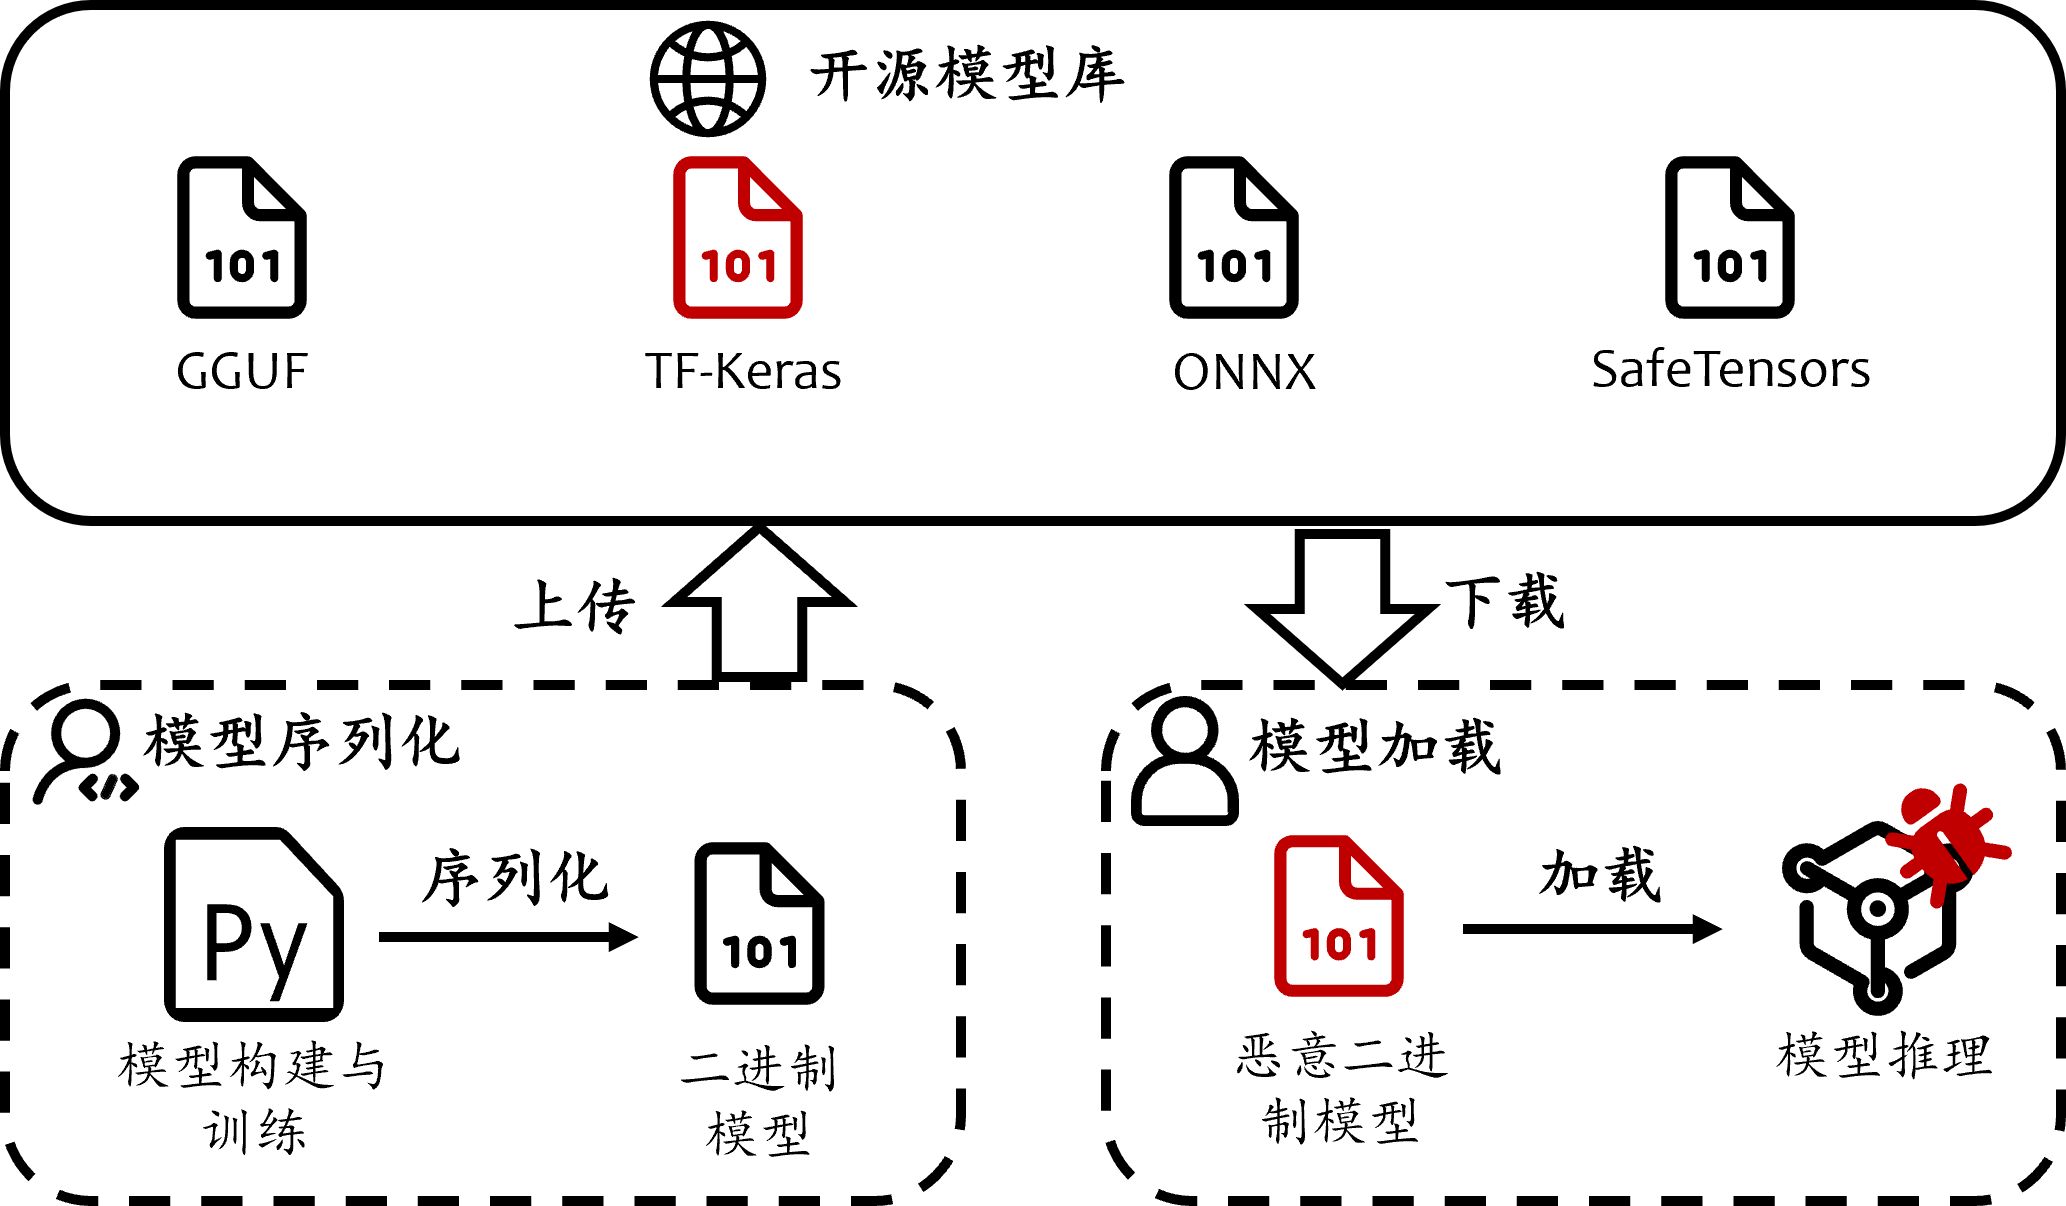
\includegraphics[width=0.8\linewidth]{figure/模型序列化与加载.png}
    \caption{\label{fig:model_serial_load}模型序列化与加载过程图}
\end{figure}

\subsubsection{模型序列化与加载}
如图~\ref{fig:model_serial_load}所示，AI 模型的生命周期通常包括模型序列化与模型加载两个关键阶段。这两个阶段构成模型供应链流转的核心路径，也是潜在安全风险产生的重要环节。

\textbf{模型序列化过程。}
模型序列化是指将内存中已经构建完成且完成参数训练的 AI 模型，按照特定数据格式转换并持久化为二进制文件的过程。该二进制文件可通过既定协议（例如 \code{pickle} 或 \code{Protocol Buffers（Protobuf）}协议）进行解析，并在后续阶段恢复至内存中执行。在 \code{TensorFlow} 框架中，主流的模型序列化格式包括 \code{SavedModel} 与 \code{HDF5}。

具体而言，模型序列化过程通常包括以下步骤：首先，开发者通过框架提供的前端 API 构建模型的层级结构，定义各层之间的输入输出关系；随后，经由框架编译器对模型图进行优化与转换，生成内存中的计算图结构；接着，利用训练数据集对模型进行参数训练与调优，使其性能指标达到预期目标；最终，通过模型保存相关 API，将训练所得的权重与偏置写入参数文件，并将模型结构序列化为图结构文件，最终实现模型序列化。在该过程中，构建模型时调用的部分 Python API 会被转换为计算图中的原子操作（Operation，Op）。在模型推理阶段，后端运行时系统将根据 Op 的名称及其属性信息，调度相应的后端 Op kernel 实现函数对输入张量进行处理，生成输出并传递至下一个 Op 节点。然而，并非所有前端 API 均可映射为后端 Op。对于无法转换为对应后端实现的 API，框架在模型序列化阶段会自动忽略相关调用逻辑。因此，并非所有 API 均具备“可持久化”特性，即并非所有 API 调用都能够被保存至模型文件中。模型完成序列化后，开发者通常将生成的二进制模型文件上传至开源模型库以供共享与复用。

\textbf{模型加载过程。}
模型加载是指将已序列化的二进制模型文件恢复至内存结构的过程。该过程不仅需要重建模型的计算图结构，还需恢复模型的参数信息。用户或开发者可从开源模型平台下载预训练模型文件，并调用框架提供的加载函数，将模型结构与参数重构为序列化前的内存状态，从而执行模型推理或继续训练。模型加载机制支持用户利用预训练模型进行迁移学习，从保存的检查点恢复训练进度，或在不同运行环境之间实现模型部署迁移。

\textbf{模型序列化与加载的潜在威胁。}
然而，在模型序列化与加载过程中，模型以二进制形式分发，其内部计算图结构及各个 Op 的具体行为对使用者而言通常不可见。与此同时，模型开源平台通常鼓励用户直接下载并运行预训练模型，而缺乏默认的沙盒隔离或安全审计机制。这种结构与执行过程的不透明性为攻击者提供了可利用空间，使其能够在模型内部嵌入恶意逻辑或异常行为，在加载或推理阶段触发潜在攻击，进而引发数据泄露或其他安全风险。如图~\ref{fig:model_serial_load}所示，恶意的开发者可以将构造的恶意模型上传到开源模型库中进行伪装，用户在毫不知情的情况下按照开元模型库的指引下载模型并直接运行推理过程，从而导致用户遭受恶意的攻击。因此，对模型序列化与加载机制进行深入理解，是分析模型供应链安全威胁与制定防护策略的基础。

\subsubsection{TensorFlow Op 注册机制}
\code{TensorFlow} 采用前后端解耦的 Op 注册机制，以支持跨平台执行及对多种硬件加速器（如 CPU、GPU 与 TPU）的高效调度。该机制主要包括 Python 前端接口、Op 注册定义机制以及 Op Kernel 实现机制三个组成部分。

\textbf{Python 前端接口。}
Python 前端接口是用户构建模型时最主要的交互层。由于 Python 语言具备良好的可读性与开发效率，其成为 AI 应用开发的主流语言。用户通过 Python 接口定义模型结构与数据流关系，而每一个前端 API 本质上是对底层 Op 的封装，使开发者能够以更抽象的方式构建计算图。
在实现层面，Python 前端接口通过跨语言调用机制与 C++ 后端交互。当前端 API 被调用并完成图构建与编译后，框架将在模型图中创建对应的 Op 节点及其张量输入输出关系。例如，当用户调用 \code{tensorflow.add} 构建模型时，在计算图中将生成一个名为 Add 的 Op 节点，并建立两条输入张量边与一条输出张量边。需要说明的是，尽管 Python 是主要前端接口语言，但理论上其他语言（如 Java）亦可实现类似封装接口，其核心功能在于构造模型图结构并触发底层 Op 注册逻辑。

\textbf{Op 注册机制。}
在 \code{TensorFlow} 中，Op 由输入张量、输出张量及其属性共同定义。在后端 C++ 源码中，框架通过 \code{REGISTER_OP} 宏完成 Op 的注册。该宏定义了 Op 的名称、输入输出张量的类型与形状约束，以及所需属性信息。输入与输出必须为张量类型，而属性类型可为 \code{string}、\code{int}、\code{float} 等多种常用数据类型。
例如，\code{REGISTER_OP("CustomOp"). Input("input:int").Output("output:float")} 宏定义了一个名为 \code{CustomOp} 的操作，其输入为整数张量，输出为浮点张量。该注册机制实现了前端接口与后端执行逻辑的解耦，使得同一 Op 定义可以对应多个不同设备的实现，从而提升框架的可扩展性与跨平台能力。

\textbf{Op Kernel 实现机制。}
Op Kernel 是指在模型运行阶段，对输入张量执行具体计算逻辑的底层实现。不同硬件加速设备（如 CPU 或 GPU）通常对应不同的 Kernel 实现，以充分利用硬件加速能力。
在 \code{TensorFlow} 中，Op Kernel 通过继承 \code{OpKernel} 类并重载其 \code{Compute} 函数进行实现。该 \code{Compute} 函数以 Op 的输入张量为参数，执行具体运算逻辑，并生成对应输出张量。完成实现后，开发者需通过 \code{REGISTER_KERNEL_BUILDER} 宏将 Kernel 注册至框架的 Op 管理系统，同时指定 Op 名称、目标设备类型以及具体实现类。例如，TensorFlow 通过在源码中声明 \code{REGISTER_KERNEL_BUILDER(Name("CustomOp"). Device(DEVICE_GPU), CustomOpClass)} 宏为 \code{CustomOp} 注册在 GPU 设备的加速实现，并且实现运算的代码在类名为 \code{CustomOpClass} 的 \code{Compute} 函数中。当模型在 GPU 上执行推理时，运行时系统将调度该类的 \code{Compute} 函数对张量数据进行处理。

通过上述前端 API 封装、Op 注册与 Kernel 实现机制的设计，\code{TensorFlow} 构建了高度模块化与可扩展的计算图执行体系。然而，这种灵活的注册与调度机制在提升框架能力的同时，也为后续章节所讨论的原生 API 能力滥用问题埋下了潜在风险基础。

\subsection{研究动机与现状}
AI 系统模型框架层的供应链正持续面临来自开源模型库中恶意 AI 模型的潜在威胁。然而，针对 \code{TensorFlow} 等框架中原生 API 所具备的隐藏能力，以及攻击者如何滥用该类能力构造恶意模型的系统性研究仍相对匮乏。现有研究多集中于模型参数层面的隐写与序列化机制漏洞利用，而对框架合法 API 在执行语义层面的安全边界缺乏深入分析。因此，有必要从模型框架层出发，对 API 能力滥用所带来的供应链风险进行系统建模与实证研究。
\subsubsection{威胁模型}
在本研究的威胁模型中，攻击者为开源模型库中的模型提供者，其能够向任意公开模型平台上传 AI 模型文件，并通过功能描述、标签或使用示例等方式诱导用户下载使用。具体而言，攻击者可利用 \code{TensorFlow} 和 \code{Pytorch} 等框架提供的合法 API 构建包含恶意逻辑的模型，并将其以二进制格式上传至如 \code{Hugging Face} 等开源模型平台。受害者通常基于功能需求搜索并下载模型文件，并在本地应用环境中直接加载与运行该模型。
在模型推理阶段，模型计算图中嵌入的合法 API 将被正常调度执行，从而触发预先组合构造的攻击行为。该过程对用户透明，即模型在向用户或上层程序返回正常推理结果的同时，隐蔽执行恶意操作。值得强调的是，攻击者无需利用传统系统漏洞，也无需提交模型源代码，仅需上传序列化后的二进制模型文件即可实施攻击。这一假设符合当前开源模型平台普遍允许用户直接上传与分发模型文件的实际情况。

本研究进一步假设，用户按照开源模型平台的官方指导，使用 \code{TensorFlow} 等框架提供的标准加载 API 进行模型加载，并以普通用户权限运行 AI 应用程序，而非以系统管理员权限执行。这一设定符合现实场景中用户通常通过 Python 脚本直接运行模型的操作习惯。此外，攻击者在攻击前并不掌握受害者的具体本地环境信息，例如本地 IP 地址、目录结构或具体文件路径等。
在上述约束条件下，攻击者的目标包括但不限于：窃取受害者本地敏感信息、篡改本地配置文件，甚至进一步获取本地系统的执行权限。该威胁模型强调，在不依赖底层漏洞利用的前提下，仅通过滥用框架合法 API，即可对模型使用者构成实质性安全威胁。
% \begin{figure}[t]
%     \centering
\begin{lstlisting}[%
    float=t,
    caption={model.py - 一个实现窃取本地文件的恶意 AI 模型例子},
    label={code:file_leak_example},
    language=python,
    emph={FixedLengthRecordDatasetV2, matching_files, DebugIdentityV3},
    emph={[2]filenames, record_bytes, input, tensor_name, debug_urls}
]
class SimpleLinearModel(tf.Module):
    def __init__(self):
        self.a = tf.Variable(3.0)

    @tf.function
    def __call__(self, x):
        # 步骤 1: 获取用户系统信息，构造文件路径
        path = tf.io.matching_files("/home/*")[0]
        path += "<target file>"  

        # 步骤 2: 滥用 API 读取目标文件
        a = tf.raw_ops.FixedLengthRecordDatasetV2( filenames = path, record_bytes = 1, ... ) 
        
        all_content = ""
        for ch in iter(DatasetSource(a)): 
            all_content += ch 

        # 步骤 3: 将文件传递给远端服务器
        tf.raw_ops.DebugIdentityV3(input = all_content, tensor_name = "test_tensor", debug_urls = ["grpc://0.0.0.0:1111"], ...)
        return self.a * x
\end{lstlisting}
% \end{figure}

\subsubsection{研究动机}
为说明系统性分析框架提供 API 隐藏能力的必要性，本节给出一个基于 \code{TensorFlow} 合法 API 构造的恶意模型示例，该模型实现了任意文件泄露攻击，如代码~\ref{code:file_leak_example}所示。该示例用于说明攻击者可在不修改底层框架代码的情况下，仅通过合法 API 组合实现数据外泄行为。该模型在序列化为二进制格式后，能够绕过 \code{Hugging Face}、\code{TensorFlow Hub} 以及 \code{ModelScan} 等现有检测机制。本研究将此类攻击统一定义为 \code{TensorAbuse} 攻击。其设计主要基于一个关键发现：\code{TensorFlow} 提供的部分合法 API 在语义层面具备隐藏的系统能力，这些能力在特定参数构造下可被滥用于实施恶意行为。以代码~\ref{code:file_leak_example} 为例，\code{FixedLengthRecordDatasetV2} 在构造其 \code{filenames} 参数后可读取指定路径下的任意文件内容；\code{DebugIdentityV3} 在设置 \code{input} 与 \code{debug_urls} 参数后，可将任意张量数据发送至远端服务器。基于上述能力，实现任意文件泄露攻击通常包含三个步骤。

第一步，如代码第 8--9 行所示，利用 \code{matching_files} API 枚举受害者系统中指定路径下的文件或目录信息，从而辅助构造目标文件路径。第二步，如第 12--16 行所示，滥用 \code{FixedLengthRecordDatasetV2} API 读取目标文件内容，并将其逐字节拼接为张量数据。第三步，如第 19 行所示，调用 \code{DebugIdentityV3} API，将构造完成的张量通过 \code{grpc} 协议发送至攻击者控制的远端服务器。攻击者在远端部署的服务端程序即可接收并重组受害者本地文件内容。该攻击方式可进一步扩展，用于遍历并泄露受害者本地的多个敏感文件。

由于 AI 模型以二进制形式分发，内部包含大量参数与复杂计算图结构，普通用户难以直接解析其具体执行逻辑，导致模型中嵌入的恶意行为具备较强隐蔽性。此外，该攻击完全基于框架原生合法 API 实现，在代码层面并未引入外部恶意模块，仅在行为语义上具备攻击属性。因此，传统基于恶意代码特征匹配或黑名单机制的检测方法难以识别此类攻击。同时，基于模型结构可视化的工具，例如 \code{TensorBoard} 或 \code{Netron} 等仅展示计算图拓扑结构，无法对 API 的具体执行语义进行安全审计~\cite{tensorboard,netron}。
从模型性能影响角度来看，此类攻击对模型精度几乎不产生可观测影响。在结构层面，仅在包含成千上万个 Op 的模型计算图中额外插入少量合法 Op，其结构变化比例通常低于 1\%。这一特性进一步增强了 \code{TensorAbuse} 攻击的隐蔽性与现实可行性。

\subsubsection{研究现状}
本节从恶意模型攻击方法与恶意模型检测技术两个方面，对当前研究现状进行分析。

\textbf{恶意模型攻击。}
现有将 AI 模型作为恶意载体的攻击方法主要包括三类：基于模型参数嵌入恶意负载、利用不安全序列化格式以及基于 \code{lambda} 层嵌入任意代码执行逻辑。

第一类方法通过修改模型参数实现恶意负载嵌入。例如，将恶意二进制数据编码至浮点数的最低有效位（Least Significant Bit，LSB）或模型属性参数中，在模型运行阶段重组并触发执行。Hua 等人提出的 MalModel 技术，通过将恶意负载编码至移动端深度学习模型权重的最低有效字节及相关结构参数中实现隐蔽存储，并在模型结构中植入并行后门分支，在特定触发样本输入时利用 Java 反射机制动态提取并执行恶意代码~\cite{hua2024malmodel}。
Tan 等人提出的 SASER 框架通过性能感知重要性指标筛选出对大模型性能影响最小的冗余参数，并利用抗量化 LSB 机制嵌入恶意负载，使其在下游模型量化压缩后仍可成功触发恶意行为~\cite{tan2025saser}。
Hitaj 等人提出的 MaleficNet 攻击框架，该方法结合扩频信道编码与低密度奇偶校验纠错技术，将恶意负载转化为微弱信号弥散嵌入神经网络权重中，并在模型加载阶段触发自我提取与执行~\cite{hitaj2024trust}。
Wang 等人提出的 EvilModel 1.0 与 2.0 框架，则通过浮点数指数位冗余及半替换策略提升嵌入容量，并利用中间层输出构造触发机制，当且仅当模型识别到特定的输入样本时，才会动态组装并执行恶意负载~\cite{wang2021evilmodel,wang2022evilmodel}。
尽管上述方法能够在模型中嵌入恶意负载，但均需修改模型参数，可能对模型推理能力产生影响，同时通常依赖特定触发器条件，攻击能力与稳定性存在一定局限。

第二类方法基于 \code{lambda} 层嵌入恶意逻辑。如图~\ref{fig:malicious_model_types} 左图所示，该方式将任意代码执行逻辑嵌入模型的 \code{lambda} 层中，在模型推理经过该层时执行恶意代码。然而，该方法主要适用于 \code{TensorFlow} 的 H5 模型格式，其他序列化格式通常不支持 \code{lambda} 层，因此适用范围有限。

第三类方法利用不安全序列化机制，尤其是基于 \code{pickle} 的反序列化漏洞。如图~\ref{fig:malicious_model_types} 右图所示，攻击者可构造包含特定 \code{pickle} 操作码的模型文件，在加载阶段触发任意函数调用。Liu 等人提出了 PickleCloak 框架利用 \code{pickle} 虚拟机底层语法特性，通过字符串混淆与隐式触发机制隐藏恶意负载~\cite{liu2025art}。然而，由于 \code{pickle} 反序列化不安全问题已被广泛认知，主流开源模型平台已部署相应检测机制，因此此类攻击较易被识别。

\begin{figure}[t]
    \centering
    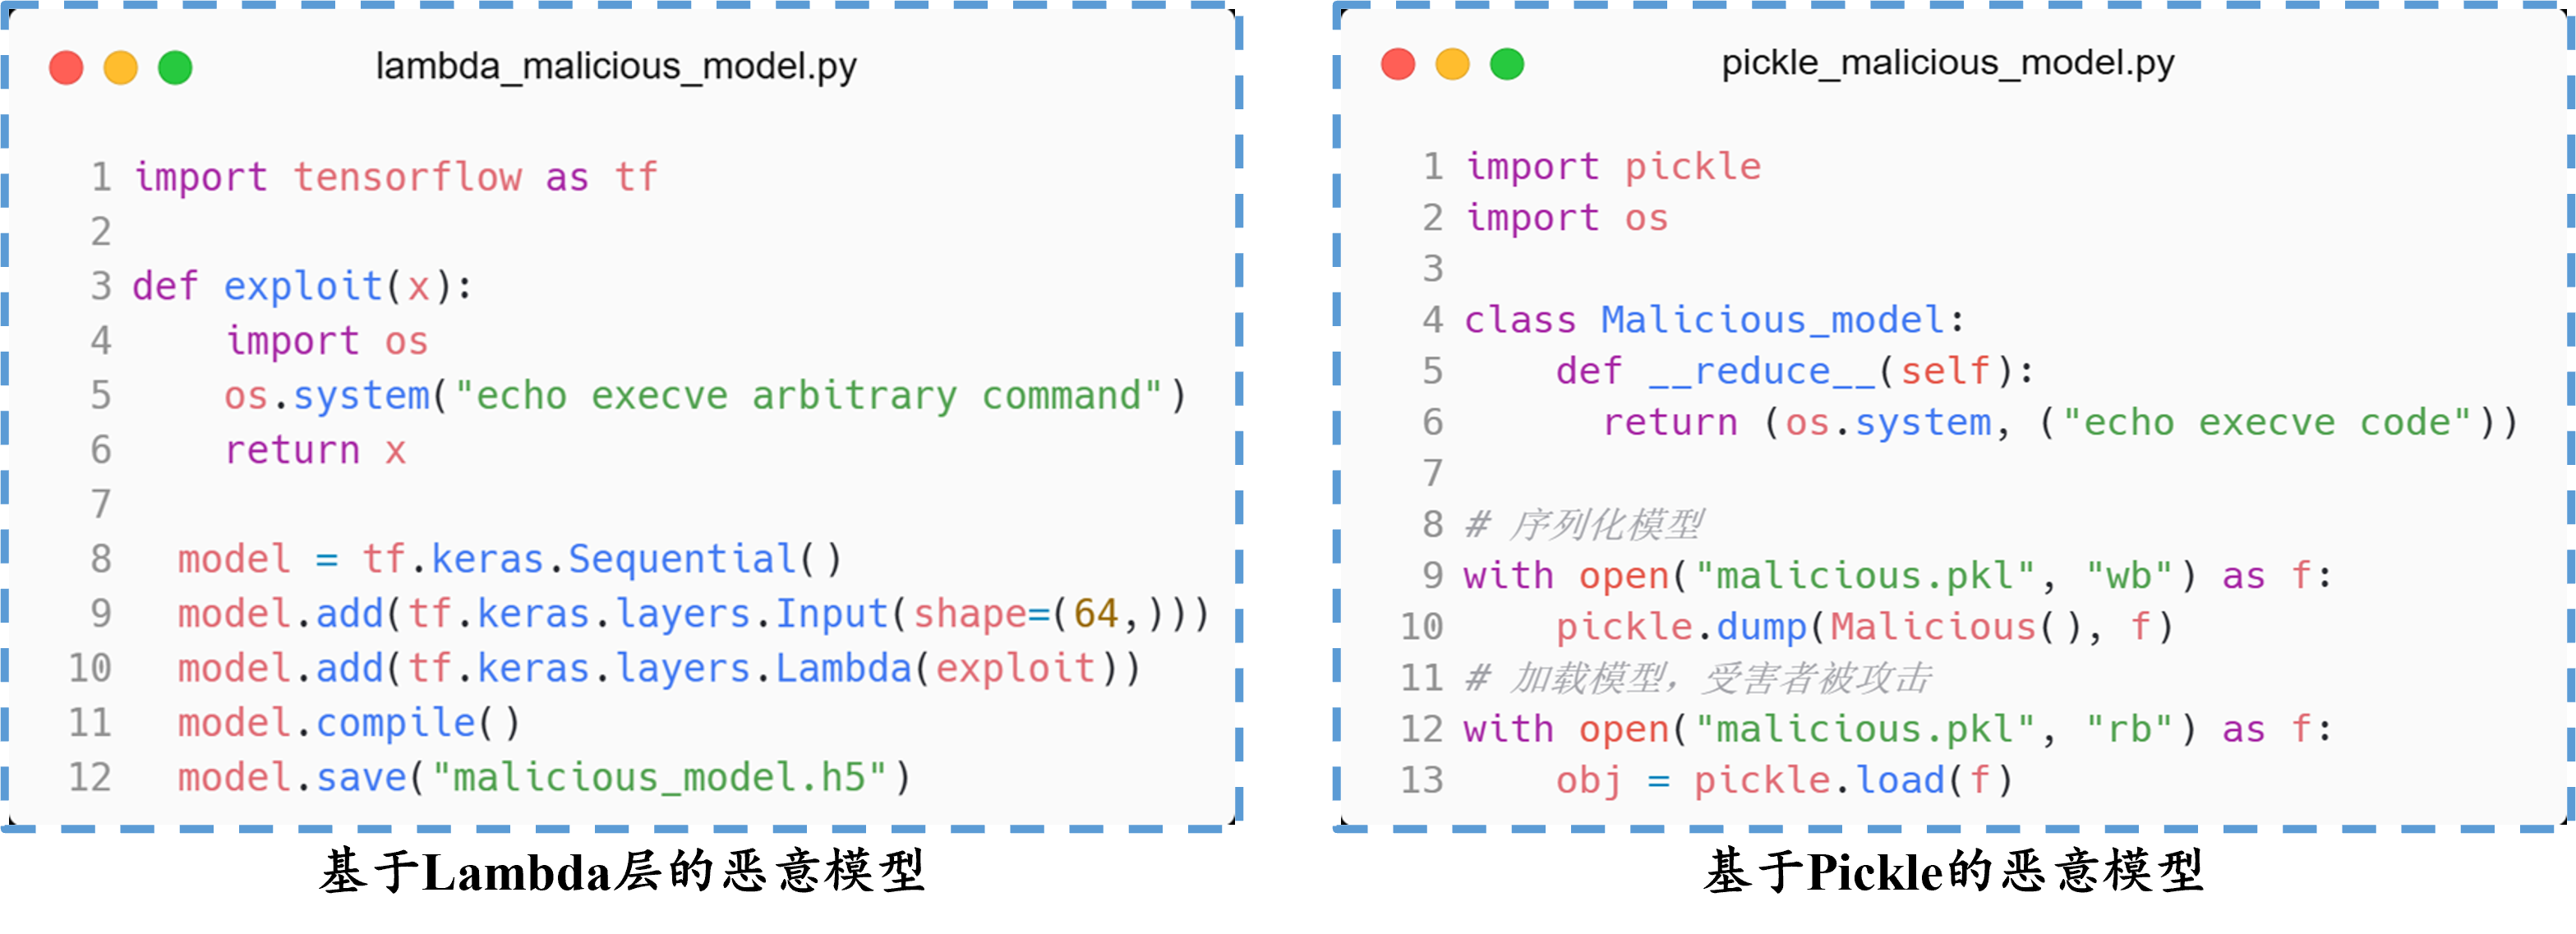
\includegraphics[width=\linewidth]{figure/恶意模型种类.png}
    \caption{\label{fig:malicious_model_types}基于 lambda 层和基于 pickle 的恶意模型例子}
\end{figure}

\textbf{恶意模型检测。}
现有恶意模型检测技术主要围绕 \code{PyTorch} 模型设计，并基于其采用 \code{pickle} 序列化机制的安全风险展开。Kellas 等人提出的 PickleBall 框架，通过静态分析机器学习库生成自定义允许列表策略，并在加载阶段动态执行严格策略，从而拦截嵌入于恶意 \code{pickle} 模型中的任意代码执行负载~\cite{pickleball}。此外，\code{pickletools} 可对 \code{pickle} 文件进行反汇编与结构化展示，以辅助识别可疑函数调用~\cite{python3123pickletools}。\code{Fickling} 提供了对 \code{pickle} 对象的反编译与静态分析能力，可检测并注入恶意负载~\cite{fickling_defcon_2021}。\code{Picklescan} 亦具备类似检测功能~\cite{picklescan}。目前较为先进的模型检测工具 \code{ModelScan} 支持识别多种框架模型中的恶意行为，包括 \code{PyTorch} 与 \code{TensorFlow} 模型~\cite{modelscan_github_2024}。此外，\code{Hugging Face Hub} 已通过其 \code{pickle} 检测机制识别出大量恶意 \code{PyTorch} 模型~\cite{montalbano2024hugging,huggingface2022pickle}。

综上所述，现有检测技术主要针对不安全序列化机制或显式代码注入场景，对于基于框架合法 API 滥用、在执行语义层面构造恶意行为的 \code{TensorAbuse} 攻击尚缺乏有效检测手段。在代码~\ref{code:file_leak_example}中本研究仅展示了利用三个TensorFlow api的文件泄漏攻击。然而，TensorFlow 框架不仅提供了数千个api，这些api相关的安全风险在很大程度上仍未被探索。通过这些 API 构造 TensorAbuse 攻击的潜力仍然未知。因此，本研究系统地研究了TensorFlow API 的功能及其构造 TensorAbuse 攻击的风险，旨在全面了解 API 及其功能的潜在威胁。


\section{TensorAbuse 攻击分析框架技术设计概览}
针对模型框架层面的 TensorAbuse 攻击问题，本研究设计并实现了一套系统化的分析框架。该框架旨在系统性地评估框架 API 所提供的隐藏能力及其可能造成的衍生威胁，从而支撑全面、大规模的攻击构造与针对该攻击的防御手段。围绕上述目标，本节首先剖析在分析 \code{TensorAbuse} 攻击能力时所面临的核心技术挑战，进而详细阐述为克服这些挑战而提出的关键技术设计。

\subsection{面临挑战}
在利用特定框架 API 构造 TensorAbuse 攻击模型的过程中，核心困难主要体现在以下两个方面。

\textbf{可持久化 API 列表的自动提取困难。}
构建稳定可复现的 TensorAbuse 攻击模型，前提是恶意载荷所依赖的 API 必须能在模型序列化过程中被完整保存至二进制文件中，并在加载阶段被成功反序列化与恢复。然而，该序列化机制对开发者而言是高度不透明的。在序列化阶段，大量无法被映射为底层计算图节点的 API 会被框架引擎自动剔除；例如，传统的 \code{os.system} 和 \code{subprocess} 等常用于执行恶意负荷的操作系统级调用，均无法在序列化过程中得以保留。因此，攻击者必须依赖那些能够以计算图形式持久化的 API。

根据 TensorFlow 官方文档，其对外提供了上千个 Python 层 API，但文档并未明确区分哪些 API 可以被保存至模型文件，亦未给出可序列化 API 所需满足的形式化规则~\cite{Tensorflowdocs}。若采用人工方式逐一测试每个 API 的可持久化能力，不仅需要为每个接口构造合法输入参数，还需验证模型保存与加载阶段的行为一致性，整体成本极高且难以扩展。此外，目前亦不存在权威指南或公开资源系统性地标识可持久化 API。例如，初步测试表明常用接口 \code{tf.io.gfile.exists} 就无法被序列化保存至模型文件中。因此，有必要设计一种自动化技术，以高效、准确地识别并提取能够嵌入模型的持久性 API。


\textbf{自动化分析 API 隐藏能力的复杂度极高。}
即便能够识别可持久化 API，其内部是否包含可被滥用的隐含能力仍然难以判断。
首先，部分 API 的实际行为与其命名语义存在显著偏差，正如代码~\ref{code:file_leak_example} 所示的 \code{DebugIdentityV3} 函数，其设计初衷是用于张量调试，然而本研究深入分析发现，该 API 在建立远程调试通道的同时，还具备向远程服务器发送数据的能力，攻击者可轻易利用此能力实施敏感文件发送实现敏感信息外泄。
其次，\code{TensorFlow} 框架的实现复杂性显著增加了能力分析难度。其体系结构采用了前后端解耦与跨语言调用的架构设计，在前端使用 Python API 构建计算图，后端以 C++ 实现算子与算子内核，且在 C++ 侧深度运用了继承、多态及宏定义等高级语言特性，导致代码逻辑高度抽象化。即便部分算子实现相对简单，若需对上千个 API 逐一进行人工代码审计，也在实践中难以实现。最后，官方文档的语义描述往往仅描述接口的输入输出与参数语义，并未完整揭示其底层资源访问行为~\cite{weimisuseapi2024}。以 \code{tf.raw\_ops.ImmutableConst} API 为例，其文档宣称该接口用于“从内存区域中读取不可变张量”~\cite{tensorflowtfrawopimmutableconst}，但本研究通过分析其底层 C++ 实现确认，该 API 同样具备直接读取本地文件系统的能力。综上所述，实现高精度、快速的 API 隐藏能力自动化提取是一项极具挑战性的任务。

\textbf{分析不同的API中具备的隐藏能力非常困难。}
即使知道了哪些API能够保存到模型中，但是分析这些API是否具备隐藏能力，能够帮助攻击者实现TensorAbuse攻击也非常困难。首先部分API虽然在表面上采用了一个名字，但是实际他具备一些名字体现不出的能力，例如代码~\ref{code:file_leak_example}中的\code{DebugIdentityV3}函数，原本是被设计来用于Debug，但是本研究发现，它在实现远程Debug的同时，也提供了向远程服务器发送消息的能力，这样的能力能够被利用于泄漏文件内容给恶意的攻击者。
并且由于框架实现上的代码复杂性更加加剧了这一分析的困难，因为TensorFlow的实现采用了前后端解耦跨语言调用的形式前端采用Python语言，后端采用C++语言，并且代码实现上使用了C++中大量继承和多态的特性，这加剧了人为直接阅读并分析代码的难度，即使部分代码实现较为简单能够分析出来，但是上千个API都手工进行分析也是不现实的。最后，虽然API的文档提供了这些API功能和参数信息，但是这些描述不仅不完整，也无法体现其正确的隐藏能力，例如\code{tf.raw_ops.ImmutableConst}这个API，在文档中说明了它可以用于从内存区域中读取张量，然而本研究分析发现它也能够被用于读取文件~\cite{weimisuseapi2024,tensorflowtfrawopimmutableconst}。综上所述，需要准确快速分析API中的隐藏能力是一个非常有挑战的事情。

\subsection{具体设计}
为系统性应对上述两大挑战，本研究设计并实现了两项核心分析技术：其一为 \code{PersistExt} 技术，用于从庞大的框架源码中自动化、大规模地提取持久化 API 及其完整调用链源码；其二为 \code{CapAnalysis} 技术，旨在通过大语言模型的深度语义理解，自动化地从所提取的源码中挖掘出 API 的高危隐藏能力，从而为 TensorAbuse 攻击构造提供能力基础。

\subsubsection{PersistExt 技术设计}
鉴于 TensorFlow 文档未系统说明 API 的可持久化属性，现有工作亦未全面解决该问题，本研究设计了 \code{PersistExt} 技术以自动识别持久性 API。该技术首先通过源码分析总结持久化 API 的结构特征，在此基础上构建自动化提取流程，从 Python 前端与 C++ 后端两个维度收集相关源码，并最终建立二者之间的精确映射关系，其整体流程如图~\ref{fig:PersistExt_design} 所示。

\begin{figure}[t]
    \centering
    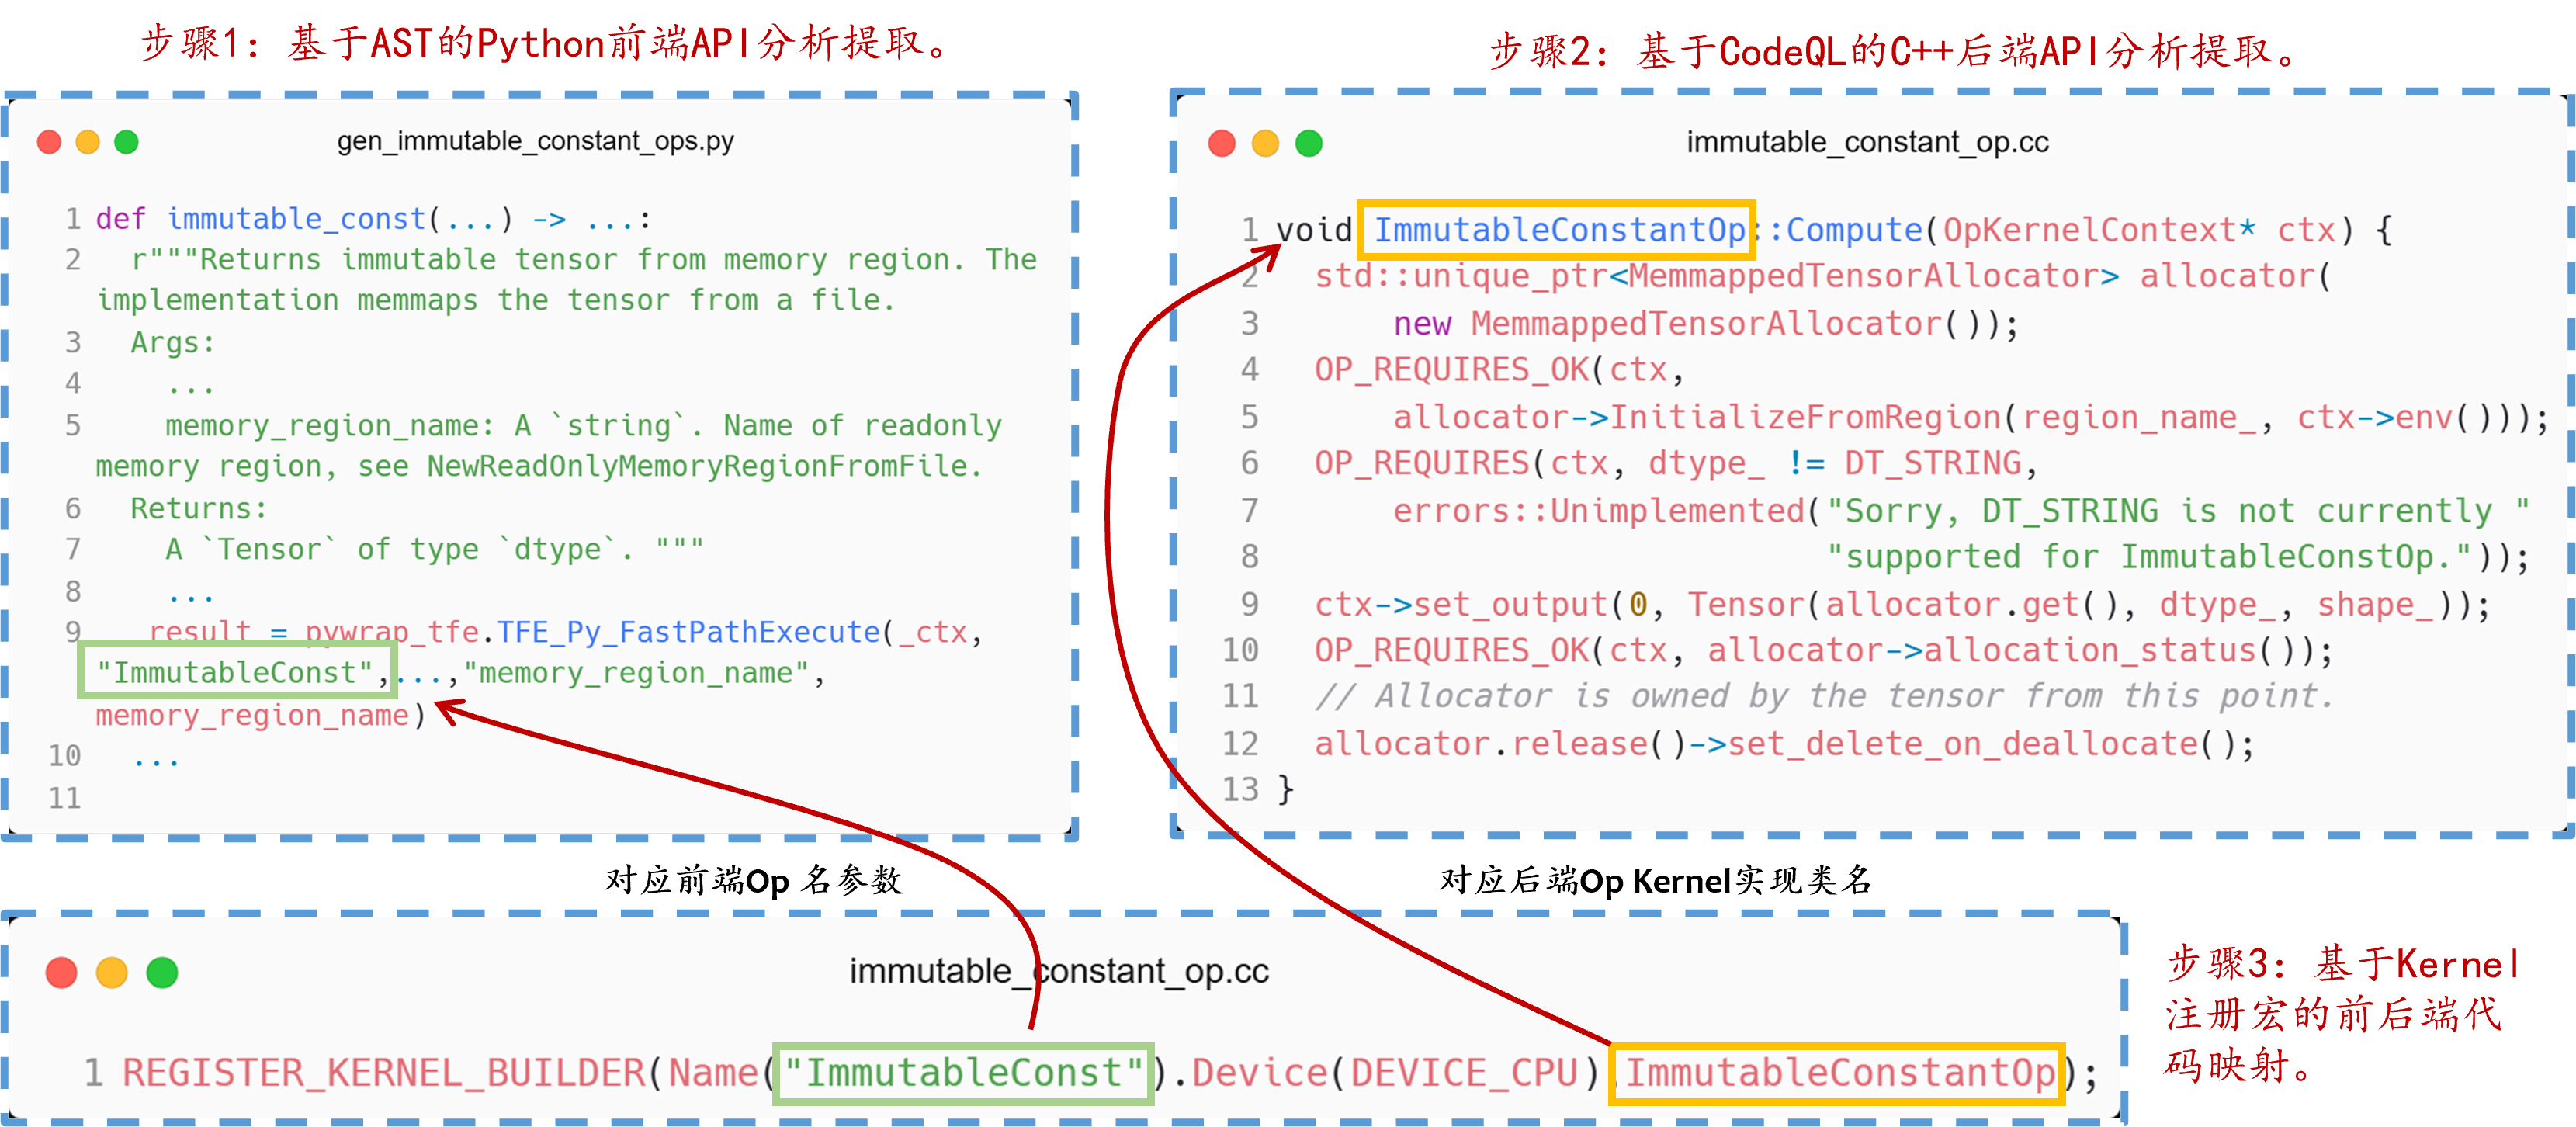
\includegraphics[width=\linewidth]{figure/PersistExt技术.png}
    \caption{\label{fig:PersistExt_design}PersistExt技术设计}
\end{figure}

\textbf{持久性 API 特征分析。}
尽管 TensorFlow 未显式定义持久性 API 的集合，但本研究通过对 \code{TensorFlow} 模型序列化相关源码逻辑可以观察到具备持久化能力的 API 在其实现路径上必然呈现出特定的跨语言调用模式。具体而言，\code{TensorFlow} 在将模型序列化为 \code{Protobuf} 格式时，不仅持久化静态的张量权重，还需固化由底层操作符构成的有向无环计算图。在模型加载阶段，系统首先恢复计算图结构，再根据当前执行环境（如 CPU 或 GPU）绑定对应的算子内核实现并运行。这意味着，一个 API 若能被成功持久化并被反序列化引擎识别，其在底层必然映射至计算图中的某个 Op 节点，并拥有至少一个具体的 C++ Kernel 实现。
正如 TensorFlow 原始论文描述，其前端 API 采用 Python 实现，而后端算子内核基于 C++ 实现，两者之间通过跨语言绑定机制连接~\cite{abadi2016tensorflow}。
基于该机制分析和代码阅读，本研究识别出三个关键跨语言接口函数：其一为 \code{pywrap_tfe.TFE_Py_FastPathExecute}，该函数通过 \code{Pybind11} 调用底层 C++ 实现~\cite{pybind11}；其二为 \code{_op_def_library._apply_op_helper}，帮助在 Python 侧构造计算节点并注入参数与属性元数据；其三为形如 \code{<API 名称>_eager_fallback} 的的回调函数簇，专门用于处理 eager 模式下的 Op 输出。凡调用上述函数之一的 Python 接口，均具备构造后端 Op 的能力，可视为潜在持久性 API。

在 C++ 后端代码层面，持久性 API 同样呈现出显著结构特征。后端计算逻辑主要通过继承 \code{OpKernel} 纯虚基类，并重写其内部的 \code{Compute} 核心方法来实现。框架要求所有合法的 Kernel 实现必须通过 \code{REGISTER_KERNEL_BUILDER} 宏向系统全局注册。该宏的展开体不仅包含了后端实现类的类名，还显式绑定了前端调用所映射的 Op 全局标识符。这一特性确立了 \code{REGISTER_KERNEL_BUILDER} 宏作为打通前后端语义屏障的关键桥梁，即宏参数中的 Op 名称锚定前端逻辑，类名称锚定后端实现。基于此特征，本研究设计了后续的自动化提取与映射方法。

\textbf{基于 AST 的 Python 前端 API 解析与提取。}
在确立了前端 Python 代码的三大调用特征后，需对 \code{TensorFlow} 庞大的 Python 源码库进行高效、准确的静态分析。传统的基于正则表达式的文本匹配方案在此场景下不仅效率低下，且极易受源码中复杂注释，例如常见的嵌套的函数使用示例或代码片段引述的干扰而产生高频误报。此外，保留并提取 API 源码中的说明性注释对于后续辅助 LLM 进行隐藏能力挖掘具有重要价值。为此，本研究摒弃了正则匹配，转而采用 Python 内置的抽象语法树解析技术。AST 能够将非结构化的文本代码转化为具有严格层次结构的树状表示，从而允许精确遍历函数声明与调用关系，完美规避注释带来的解析噪声。

具体而言，\code{PersistExt} 技术将源码树中所有 \code{.py} 文件解析为 AST 实例，随后遍历每棵树中的函数定义节点（即 \code{FunctionDef} 节点），并对其内部的函数调用子图进行深度优先遍历，以检索是否调用了前述三大特征函数。若满足条件，则将该函数标记为持久性 API 前端接口。在此过程中，\code{PersistExt} 还会同步提取传递给特征函数的参数以及该函数的文档注释。如图~\ref{fig:PersistExt_design} 步骤一所示，\code{PersistExt} 成功识别出 \code{immuatable_const} 函数，因其内部显式调用了函数 \code{pywrap_tfe.TFE_Py_FastPathExecute}。同时，通过解析该调用点提取出关键参数 \code{ImmutableConst}，其对应了 API 在静态计算图中所映射的节点名称，并保留了说明该 Op “可从文件映射张量”的注释文本，为后续推断其具备潜在文件访问能力提供了线索。

\textbf{基于 CodeQL 的 C++ 后端源码分析提取。}
鉴于 \code{TensorFlow} 的 C++ 后端包含大量宏定义、继承结构与跨文件调用关系，传统的静态代码分析工具难以有效应对。例如，LLVM 框架在前端处理阶段即会对宏进行强制展开，导致将其转换为中间表示（Intermediate Representation, IR）后，原始宏定义的语义边界完全丢失~\cite{Lattner2004LLVM}；另一方面，由于框架中的 Op 内核声明与具体实现往往散布在不同的头文件与源文件中，基于 Clang AST 的解析方案通常受限于单文件编译单元的作用域，无法处理跨文件、跨模块的深层调用分析~\cite{ClangAST}。为此，\code{PersistExt} 最终设计采用专为复杂代码库审计设计的 \code{CodeQL} 分析引擎~\cite{CodeQL}。\code{CodeQL} 支持将整个代码库编译为关系型数据库形式，允许安全研究人员使用声明式的查询语言直接对代码模式，如特定宏调用与类继承树等进行高精度数据流追踪与提取。

具体而言，\code{PersistExt} 首先构建 \code{TensorFlow} 源码的 \code{CodeQL} 数据库，随后编写定制化查询脚本，利用内置的 \code{getABaseClass} 与 \code{hasName} 关键词，全局搜索所有直接或间接继承自 \code{OpKernel} 基类的实体类，并定位其内部覆写的 \code{Compute} 方法。由于 \code{CodeQL} 默认查询仅返回目标函数所在文件的绝对路径及代码起始行号，\code{PersistExt} 进一步辅以基于堆栈逻辑的括号匹配算法，以精确截取目标函数的完整代码块~\cite{hu1999calculating}。为防止源码注释或字符串常量内存在的孤立括号对匹配算法造成语法树闭合干扰，系统额外采用了注释符和引号的匹配算法来取出注释带来的噪声。最终，该阶段成功输出了所有底层 Op 内核的 \code{Compute} 执行逻辑及其类声明信息。如图~\ref{fig:PersistExt_design} 步骤二所示，\code{PersistExt} 成功定位并完整截取了 \code{ImmutableConstantOp} 类的 \code{Compute} 成员函数代码块及其周边注释，这些代码详细封装了该算子从内存映射文件中读取数据并初始化输出张量的底层实现细节。

\textbf{基于Kernel注册宏的前后端代码映射。}
在完成前置的独立提取工作后，\code{PersistExt} 获取了包含所有可能持久化 Python API 前端声明的集合，以及所有底层 C++ Op 内核实现代码的集合。本阶段的核心任务是建立这二者间的确切映射关系，如前所述，该映射通过 \code{REGISTER_KERNEL_BUILDER} 宏实现。为此，\code{PersistExt} 再次调用 \code{CodeQL} 引擎，利用 \code{getMacroName} 关键字精准定位所有针对内核注册的宏调用实例。通过对提取语句进行词法解析，\code{PersistExt} 从中剥离出目标 Op 的全局标识符（与 Python 侧提取的 Op 名称对应）以及承载该逻辑的 Op 内核类名（与 C++ 侧提取的实现类对应）。通过构建基于 Op 标识符的哈希映射表，实现了 Python API 前端代码与底层 C++ \code{Compute} 方法的一一映射对齐。需要指出的是，由于框架支持多后端的设备加速分发设计，单一的前端 Op 标识符可能通过不同的注册宏绑定多个针对特定硬件（如 CPU 或 GPU）定制的内核类；因此，整体映射关系呈现出一对多的拓扑。如图~\ref{fig:PersistExt_design} 步骤三所示，\code{PersistExt} 解析到一个关键宏实例，该实例声明了在 CPU 硬件后端上，标识符为 \code{ImmutableConst} 的 Op 将由 \code{ImmutableConstantOp} 类负责具体的运行时计算。这一线索成功地将 Python 侧的 \code{immutable_const} API 调用与 C++ 侧 \code{ImmutableConstantOp::Compute} 函数的执行逻辑锚定在一起。

至此，\code{PersistExt} 技术实现了对框架内所有可持久化 API 列表的无损自动化提取，不仅获取了它们在模型静态计算图中对应的底层 Op 节点标识符，更完整地拼凑出前后端源码映射关系，为后续能力分析与攻击构造奠定了基础。

\begin{figure}[t]
    \centering
    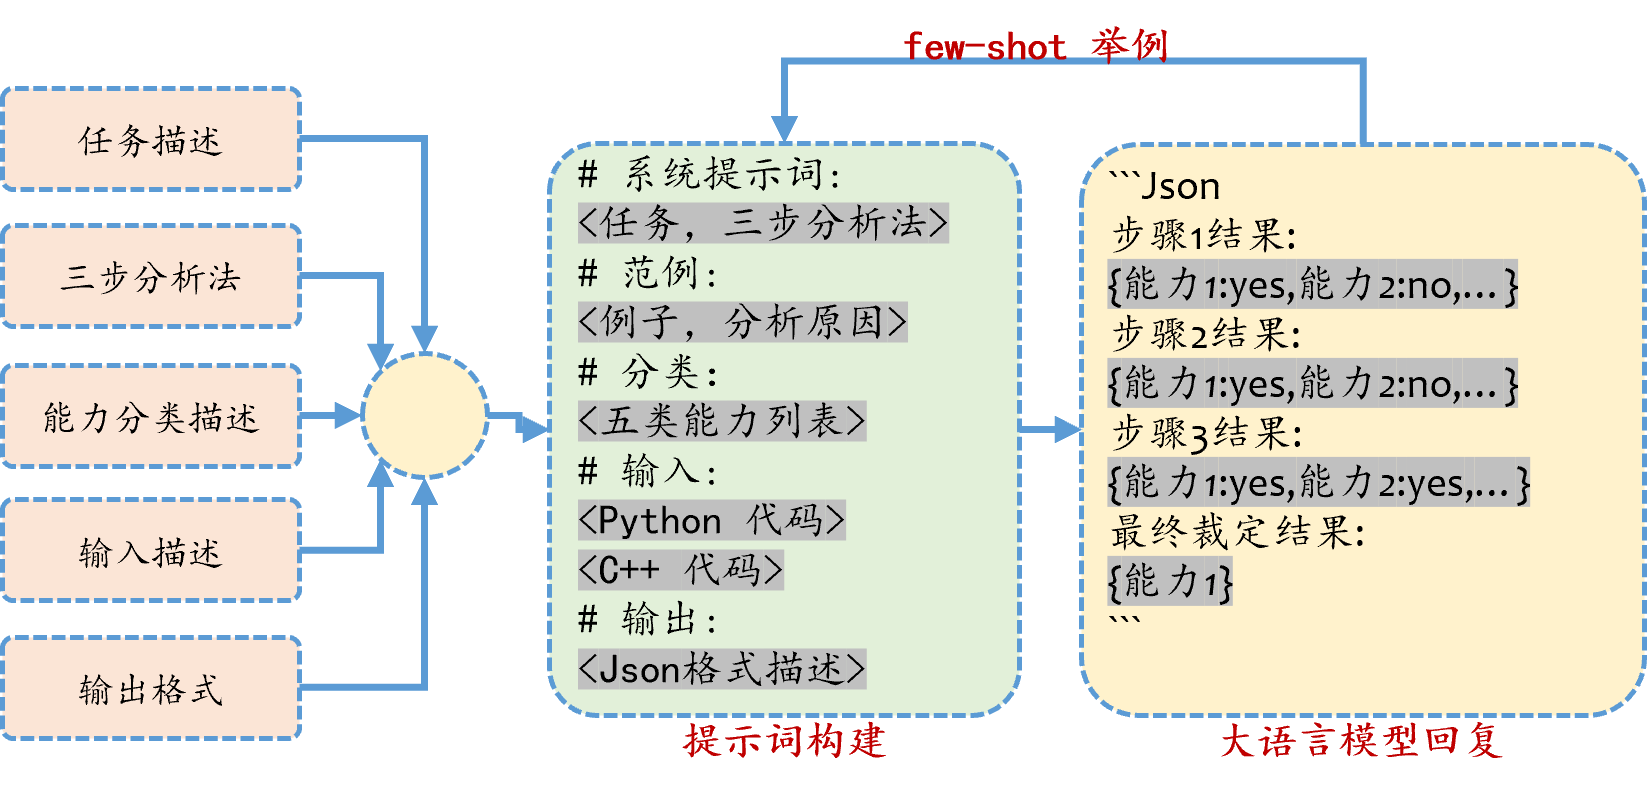
\includegraphics[width=0.9\linewidth]{figure/CapAnalysis技术.png}
    \caption{\label{fig:CapAnalysis_design}CapAnalysis技术设计}
\end{figure}


\subsubsection{CapAnalysis 技术设计}
在使用 \code{PersistExt} 技术提取出所有持久化 API 以及他们的前后端代码实现之后，由于 API 的数量繁多和代码复杂的特性，手工去分析这些 API 具备的隐藏能力仍然是一个耗时耗力的过程，不仅准确度不高容易丢失个别能力，也没法自动化地处理上千个 API。为此，本研究提出并设计了 \code{CapAnalysis} 技术，它利用了大语言模型对于代码理解的突出能力，且无需人类专家干预，即可快速理解代码的作用以及其深层次的含义，从而能快速获得 API 背后的隐藏能力的同时也和手工分析相比具备较高的准确性和效率。

根据大量的实验观察和对比发现，相比推理判断能力，大语言模型对于特定分类任务的能力似乎更加突出。为此 \code{CapAnalysis} 设计上采用让大语言模型对 API 源码分析后，完成对能力的分类任务，而不是直接将代码交给它让它分析其中具备的能力。这意味着本研究需要首先进行一个能力的实证研究和分析，探寻出 API 具备隐藏能力的列表。随后 \code{CapAnalysis} 采用结构化的方法来构建提示词，将提示词拆分成五个结构化部分，如图~\ref{fig:CapAnalysis_design}所示，这种结构化的方式有助于帮助大语言模型更好地理解任务需求，并且以固定格式进行输出，方便后续处理。而为了提高大语言模型的生成质量，\code{CapAnalysis} 还采用了多种提示词工程技术，例如使用了生成式知识技术提供背景知识；采用 Few-shot 技术给大模型提供少量案例，让其分析更加精确；还采用了思维链技术让大模型分步骤进行分析等~\cite{giray2023prompt,liu2021generated,wang2020generalizing,kuppa2023chain}。\code{CapAnalysis} 还采用了启发式探索策略，让大模型进行了两轮问询，在首轮问询中，提示词引导大模型启发式地生成详细隐藏能力，从而获取精细地隐藏能力分类列表，而在第二轮根据精细能力列表进行细致化分类，获取最终结果。

\textbf{能力分类。}
为了识别 TensorFlow API 具备能力的列表，本研究首先从 TensorFlow 官方文档中随机提取了 100 个 API 进行实证研究，该提取过程会确保 API 覆盖每一个类别，然后利用大模型对能力进行两轮提取，第一轮结果提供初步的启发式能力分类，第二轮提供了精细化能力分类，并获取到最终确定结果。

在实证研究方面，经过对随机提取的 API 代码手工分析后，本研究获得了它们能力初始分类，确定了四大类主要功能，包括：纯数学计算，文件系统访问，网络访问和进程管理。为了进一步完善这一分类，本研究下一步采用让大模型启发式地挖掘隐藏能力。具体来说，\code{CapAnalysis} 在第一轮中为了防止遗漏，给大模型的提示词是四个手工确定的粗略能力，然后要求大模型报告它识别出的任何新能力，在将第一轮的结果手工分析后表明，大模型不仅启发式地挖掘出了一个代码执行的新大类，更是将前述四个粗略能力进行了更进一步地细化，分化成了多个小类，具体分类如下所示：
\begin{itemize}
    \item 文件系统访问：文件读，文件写，目录读，目录写。
    \item 网络访问：网络发送，网络接收。
    \item 进程管理：进程创建，进程撤销，进程睡眠。
    \item 纯计算：数学计算，内部数据管理，编码和解码。
    \item 代码执行：用户可控函数执行。
\end{itemize}

而为了确保这一分类的完备性，\code{CapAnalysis} 又进行了第二轮地挖掘和分类，在这第二轮中给大模型的提示词是这 5 大类 13 小类，并同样让其挖掘新能力。然而大模型没有再报告新的能力分类，也没有挖掘出更细化的小类，因此本研究认为通过如上所述的迭代方法获得的类别便是 TensorFlow API 所具备的全部能力。

\textbf{三步分析法。}
由于分析 API 是一个复杂难题，因此 \code{CapAnalysis} 将该大难题分解成三个小步骤，让大模型采用思维链方式一步步思考，逐一判断，最后结合多步分析自主裁定，以提高其分析准确性。具体来说 \code{CapAnalysis} 将其分为注释分析、宏分析和逻辑分析三个步骤。

注释分析基于本研究对代码的观察发现 API 的 Python 部分注释通常包括对 API 参数、输入输出以及使用示例的描述，这些信息极有可能包含其关于隐藏能力的说明。因此第一步 \code{CapAnalysis} 要求大模型利用其处理自然语言的熟练程度分析代码中的注释，并提供了少量案例增强其能力：例如，注释中的字符串“server\_address: A 'Tensor' of type 'string'.”表明了 API 存在一个服务器地址相关的参数，意味着其可能存在网络访问的能力。

宏分析主要用于分析 API 的 C++ 后端代码中的宏调用，例如 \code{OP_REQUIRES} 等。这些宏负责将输入张量中的数据从跨语言上下文中解析出来并初始化，然后检查它们是否满足特定条件。值得注意的是，这些宏中的函数调用和参数名字也能提供隐藏能力的信息，例如 \code{OP_REQUIRES_OK(ctx, AppendStringToFile(file_path_, ended_msg, ctx->env()));} 宏中调用了 \code{AppendStringToFile} 函数，该函数中还有 \code{file_path_} 参数，这隐含了这个 API 或许具备文件访问的能力。\code{CapAnalysis} 同样会给大模型诸如这样的例子指导其分析宏。

逻辑分析主要是对 API 的前后端源代码进行函数逻辑判断。虽然这一步 \code{CapAnalysis} 只提供了后端 Op kernel 实现的 \code{Compute} 函数以及少量其函数调用，但是大模型仍然能给出非常准确的回答和函数分析过程，这似乎与大模型训练时采用了 TensorFlow 源码对其进行训练有关，因此其知识网络中能够补全相关函数调用。这一步中 \code{CapAnalysis} 同样会给大模型一些范例作为 few-shot 分析手段，例如，提示词中会包含“如 \code{strings::StrAppend( &error_msg, ", or file://<filename>");} 这样的函数调用表明API具有文件访问能力”的范例指引大模型。

最后大模型会根据以上三个步骤的最终结果进行综合裁定，以决定所提供 API 的最终具备的隐藏能力。例如图~\ref{fig:PersistExt_design}的代中，大模型在注释分析过程中注意到了 \code{from a file} 和 \code{NewReadOnlyMemoryRegionFromFile}字符串，这标明了该 API 会具备文件访问的能力。在宏分析中，大模型认识到宏中调用了 \code{InitializeFromRegion} 函数，且该函数调用了 \code{region_name_} 和 \code{ctx->env()} 作为参数，虽然没有显示说明其和文件访问相关，但是它读取了上下文环境信息，只能说可能具备文件访问的能力，于是大模型在这一步给出的结果为不具备文件访问能力。在最后的逻辑分析中，大模型最终确认\code{allocator->InitializeFromRegion}上下文中的函数\code{NewReadOnlyMemoryRegionFromFile} 是从文件显式初始化的，从而确认了文件读取能力。虽然 \code{CapAnalysis} 在提示词构建过程中没有将 \code{InitializeFromRegion} 函数源码 和 \code{NewReadOnlyMemoryRegionFromFile} 函数定义给出，但是大模型根据它已有的知识发现 \code{InitializeFromRegion} 函数不仅在内部调用了 \code{NewReadOnlyMemoryRegionFromFile} 函数，还对其进行初始化，从而分析出了文件访问这一准确的信息。

\textbf{系统提示词构建。}
提示词设计的好坏直接决定了大模型输出答案的质量，因此 \code{CapAnalysis} 技术精心设计了输入指令，采用 XML 结构化提示词设计来增强理解，其提示词主要包含五个主要组成部分，如图~\ref{fig:CapAnalysis_design}所示。

\begin{itemize}
    \item 系统提示词：作为TensorFlow代码专家和安全专家，我希望您使用您对TensorFlow源代码的理解，分析给定TensorFlow API的隐藏能力，我会给你的输入包括 API 的前端 Python 代码和后端 c++ Op kernel 实现代码。我希望你一步步地进行思考，第一步分析 API 的注释，第二步分析 API 的宏定义，第三步分析 API 的函数逻辑，并给每个步骤一个输出，最后根据这三个步骤的输出做一个最终裁定，确定该 API 所具备的能力。
    \item 范例：该部分给出的是上一个小节中的为三部分析法构造的 few-shot 例子以及最终裁定的例子，用以指引大模型参考范例进行分析和回答。
    \item 分类：分类部分按照前述的能力分类进行，其主要包含 5 个大类，13 个小类能力，交由大模型自主选择进行分类。
    \item 输入：输入部分为利用 \code{PersistExt} 技术提取出 API 代码，包括前端 Python 部分代码和后端 C++ 部分代码以及它们的注释。
    \item 输出：最后输出部分要求大模型按照特定的格式每个步骤每个步骤进行输出，并确定是否具备每一种能力，如果具备则该能力标注 yes，否则标 no，并且最终裁定需要给出最终的该 API 具备能力的列表。此外最后输出部分需要按照 Json 格式进行格式化输出以方便处理。
\end{itemize}

最后，将以上五个部分组合起来就形成了一个 API 的完整提示，\code{CapAnalysis} 为一千多个 API 都自动化生成了一份提示词。为进一步确保大模型能够理解任务，输出准确结果，\code{CapAnalysis} 还为其使用了三个真实人工分析的示例和回答，指导其进行学习，并且会随机添加大模型生成的回答作为后续其他提示词的 few-shot 部分。

\begin{figure}[t]
    \centering
    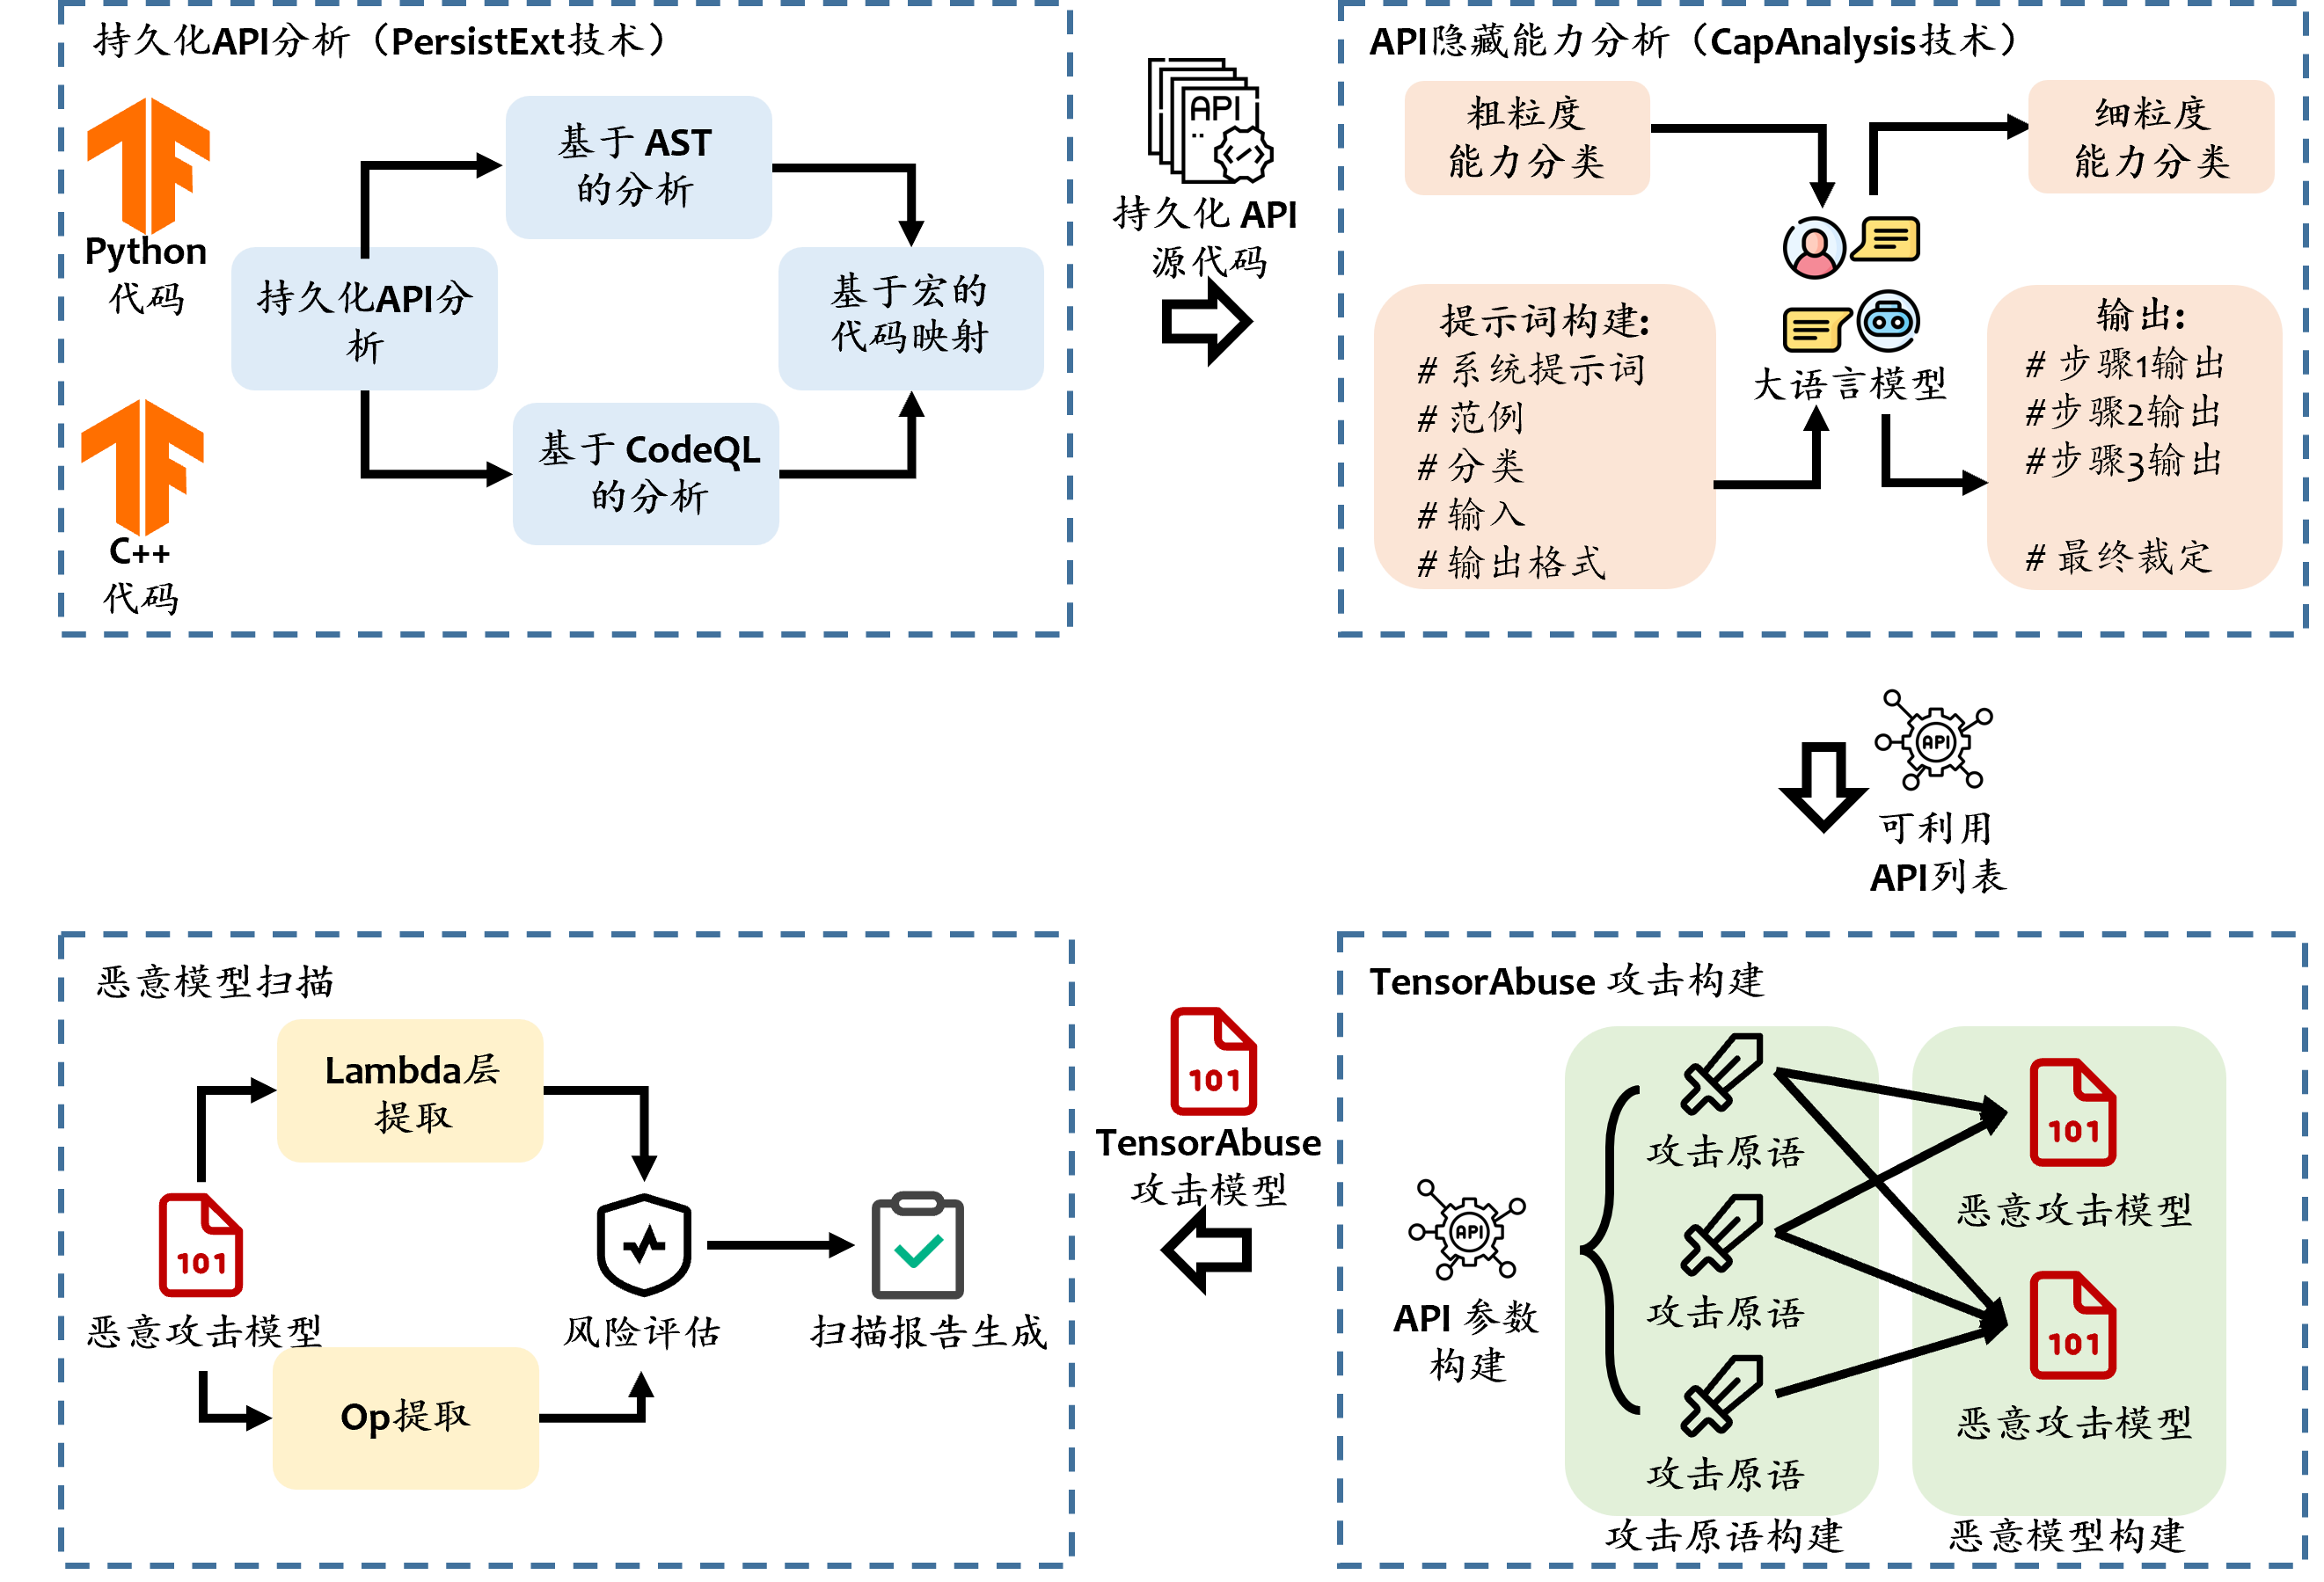
\includegraphics[width=\linewidth]{figure/TensorAbuse攻击分析框架.png}
    \caption{\label{fig:tensorabuse_imply}TensorAbuse 攻击分析框架图}
\end{figure}


\section{框架详细实现}
本小节从框架实现的角度，详细说明本研究提出的 TensorAbuse 攻击分析框架。如图~\ref{fig:tensorabuse_imply} 所示是 TensorAbuse 攻击分析框架示意图，其主要包含四个阶段，分别是持久化 API 分析，API 隐藏能力分析，TensorAbuse 攻击构建以及恶意模型扫描，四个阶段相互衔接，最终完成对 AI 系统的模型框架层中模型供应链的安全分析与防御。

\textbf{持久化 API 分析阶段。}
该阶段以 TensorFlow v2.15.0 源码作为输入，核心目标在于分析出所有能够保存到模型中的 API 列表。具体而言，该阶段主要采用了 PersistExt 技术，将源代码首先采用 \code{bazel build} 命令将其源码进行本地编译，这一过程主要原因是 TensorFlow 在代码中会利用特定模版生成新的代码文件（一般以 \code{gen_xxx_ops} 命名），然后将编译后的所有代码文件再拆分成前端 Python 代码和后端 C++ 代码，前端代码以 \code{.py} 作为后缀名，后端代码以 \code{.c， .cpp， .cc， .cu} 等作为后缀名。前端代码利用 AST 模块进行自动解析，识别出调用跨语言调用接口的函数后提取出其代码，后端利用 \code{codeql database create --language=cpp } 命令构建 TensorFlow代码 数据库，提取出所有\code{REGISTER_KERNEL_BUILDER} 宏语句和所有继承自 OpKernel 类，且成员函数带 \code{Compute}, \code{ComputeAsync} 等函数的位置信息，接着用括号匹配算法对其进行提取出源码。最后采用 宏中包括的 Op 名字和类名字将前后端代码进行映射，提取出了 1,083 个持久化 API。

\textbf{API 隐藏能力分析阶段。}
该阶段以上一阶段提取的持久化 API 前后端代码作为输入，核心目标在于分析这些 API 所具备哪些隐藏能力。具体而言，该阶段主要采用了前述的 CapAnalysis 技术，首先通过随机抽样和手工分析的方式提取出了粗粒度的能力分类，然后交由 ChatGPT-4 大模型进行多轮问询获得细粒度的完备的能力分类列表。随后利用该分类列表以及 API 源码，构建了大模型提示词，交由大模型按步骤审查多轮，最终获得了所有 1083 个持久化 API 所具备的能力，其中 150 个 API 可能存在恶意能力，能够被攻击者所利用。

\textbf{TensorAbuse 攻击构建阶段。}
该阶段以上一阶段提取的 150 个可能能够被利用的 150 个“恶意” API 作为输入，核心目标在于构建出能够实现 TensorAbuse 攻击的恶意模型。具体来说，该步骤为这些 API 构建了不同的参数，从而使其被调用时能够触发特定的能力，形成特定的攻击原语。这些攻击原语可以以 SavedModel 格式嵌入到任何 TensorFlow 模型中，并在用户执行模型推理时触发。然后利用这些攻击原语，通过对它们按照特定顺序进行组合，即可实现强大的恶意 TensorAbuse 攻击。本研究在这阶段将这些攻击嵌入进 Yamnet 模型中（在模型正常逻辑代码中添加特定 API 的调用组合），并将其上传至 Hugging Face 以检测这些恶意攻击能否绕过网站的检测，结果显示。

\textbf{恶意模型扫描阶段。}
经过上一阶段本研究发现目前最先进的工具并无法检测出 TensorAbuse 攻击这种新型攻击，为此本研究开发了一个恶意模型检测工具来识别此类威胁。具体而言，该工具的核心思想是通过分析模型结构中的 Op 列表及其调用参数来检测潜在的恶意行为。对于给定的一种 TensorFlow SavedModel 格式的模型，该工具利用 TensorFlow 内置的解析工具将其二进制文件转换为模型图结构，这个静态模型图中包含了所有被调用的算子信息及其参数。对于算子信息，该工具扫描是否存在与前面分析出的威胁 API 对应的算子名称。如果找到这些算子，模型便可能处于风险之中。接着，该工具进一步检查这些可疑算子的参数，尤其关注以 base64 编码的字符串类型张量，这些字符串张量往往包含指向敏感系统文件或未知IP地址的路径，如果发现这样的恶意参数，便将该模型归类为恶意。此外，本研究还使用检测工具扫描了托管在 HuggingFace 上的 3,000 多个模型。虽然我们发现了24个使用潜在可利用API的模型，但其参数中未发现恶意行为。

\section{实验评估}
本小节对 TensorAbuse 攻击分析框架的核心技术以及构造的攻击进行了系统性地分析和评估。具体而言，本研究利用 TensorFlow 官方文档中的 API 列表作为基准，来判断 PersistExt 技术的可用性；同时构建了一个针对 API 能力分析的数据集来评估 CapAnalysis 技术的准确性。

\subsection{PersistExt 技术实验结果}
使用 PersistExt 技术，本研究提取出了大量代码片段，其中用基于 AST 的 Python 代码分析提取出了 1,585 个 Python API，其中包括了 149 个并未在 TensorFlow 官方文档列出的 API~\cite{Tensorflowdocs}。通过基于 CodeQL 的分析方法，PersistExt 从 C++ 代码中提取出了 1,246 个类是 OpKernel 类的子类，其中 1,147 个类具有 Compute 成员函数。此外，PersistExt 还从 C++ 代码中提取出了 11,221 个 \code{REGISTER_KERNEL_BUILDER} 注册宏。这种数量差距的原因主要是针对一个 Op 而言，可能会注册多个这个 Op 相关的 Op kernel。例如 \code{ArgMin} Op 为 \code{int16}， \code{int32} 和 \code{int64} 数据类型分别注册了三个内核实现，但是这三个都使用相同的模板类 \code{ArgMaxOp} 来实现它们的具体运算操作，从而这三个注册产生的都是从 \code{ArgMin} Op 到 \code{ArgMaxOp} 类的映射。最后在去重之后，PersistExt 最终提取出了 1,083 个独一无二的映射，即所需的持久化 API 和它们的代码。部分前后端代码没有形成映射，主要因为一些 Op 为测试使用的Op，因此并没有在源码中给它们注册具体实现类，还有一部分 Op 采用另外封装的宏来注册，但是这些例外情况主要都是纯计算的 Op，因此对最后构造攻击的 API 列表结果并没有产生影响。
在 PersistExt 技术准确性方面，其源代码分析采用独特的跨语言调用接口作为特征来识别 API，甚至识别出了官方文档中没列出的 Op。而在攻击构造阶段，本研究在构造参数进行攻击原语生成时，所有的 API 都被成功地保存到了模型中，也在一定程度上说明了 PersistExt 技术的准确性。

\begin{table}[t]
\renewcommand{\arraystretch}{1.5}
\caption{CapAnalysis 分析结果}
\centering
\small
\begin{tabular}{c c c c}
\hline
\cellcolor[HTML]{C0C0C0}\textbf{能力分类} & \cellcolor[HTML]{C0C0C0}\textbf{第一轮分析} & \cellcolor[HTML]{C0C0C0}\textbf{第二轮分析} & \cellcolor[HTML]{C0C0C0}\textbf{测试集分析} \\
\hline
纯计算 & 710 & 965 & 67 \\
\cellcolor[HTML]{EFEFEF}文件系统访问 & \cellcolor[HTML]{EFEFEF}71  & \cellcolor[HTML]{EFEFEF}58 & \cellcolor[HTML]{EFEFEF}18 \\
网络访问 & 28  & 25  &  9\\
\cellcolor[HTML]{EFEFEF}进程管理 & \cellcolor[HTML]{EFEFEF}52  & \cellcolor[HTML]{EFEFEF}13 & \cellcolor[HTML]{EFEFEF}1 \\
代码执行 & 3  & 54  &  8\\
\cellcolor[HTML]{EFEFEF}不确定 & \cellcolor[HTML]{EFEFEF}224  & \cellcolor[HTML]{EFEFEF}13  &  \cellcolor[HTML]{EFEFEF}6\\ \hline
API 覆盖数量 & 1083  & 1083 &  100\\
\hline
\end{tabular}
\label{table:captech_result}
\end{table}

\begin{table}[t]
\renewcommand{\arraystretch}{1.5}
\caption{CapAnalysis 抽样评估结果}
\centering
\small
\begin{tabular}{c c c c c c}
\hline
\cellcolor[HTML]{C0C0C0}\textbf{轮数} & \cellcolor[HTML]{C0C0C0}\textbf{准确} & \cellcolor[HTML]{C0C0C0}\textbf{超出} & \cellcolor[HTML]{C0C0C0}\textbf{遗失} & \cellcolor[HTML]{C0C0C0}\textbf{错误} & \cellcolor[HTML]{C0C0C0}\textbf{全部} \\
\hline
第一轮 & 70 & 10 & 1 & 19 & 100\\
\cellcolor[HTML]{EFEFEF}第二轮 & \cellcolor[HTML]{EFEFEF}83  & \cellcolor[HTML]{EFEFEF}4 & \cellcolor[HTML]{EFEFEF}4 & \cellcolor[HTML]{EFEFEF}9  & \cellcolor[HTML]{EFEFEF}100\\
\hline
\end{tabular}
\label{table:captech_evaluation}
\end{table}


\subsection{CapAnalysis 实验结果}
为了证明 CapAnalysis 技术的准确性，本研究首先构建了一个 API 能力分析的基准数据集。其从 API 列表中随机抽取了 100 个 API，并保证它们覆盖了每一个类别。本研究对这些 API 进行了大量的手工分析工作，包括静态代码分析其能力，以及动态地构建参数，运行模型后提取运行过程中的系统调用，判断其能力。随后本研究使用 CapAnalysis 对 1,083 个 API 进行两轮的能力分析，第一轮要求大模型启发式地发生新能力并报告，第二轮使用细化了之后的能力分类，最终两轮结果如表~\ref{table:captech_result}所示，其显示了两轮中和测试集中每个功能的 API 数量，部分 API 会包含多个功能。
\section{TensorAbuse 攻击评估}

\section{本章小结}